\section{Skeletal Pose Estimation}

Skeletal Tracking, even though not directly related by itself to the aims of the project, is part of the base functionality needed for the development of all core components. Skeletal tracking and pose estimation is achieved by the Kinect Skeletal API, which uses the Kinect's depth feed.\\

Detecting humans, possibly in different poses, has been an interesting point of research in different areas. Aiming to detect human activity in real time, A. Argyros and M. Lourakis \cite{Argyros2004}, developed a method for tracking multiple skin-coloured objects, which could represent human parts such as the face and the hands. Simply using colour detection raised some issues when detecting different body parts intersecting with each other, as they could be interpreted as a single object. This issue was addressed by detecting each object as it entered the field of view of the camera and assigning a unique label to it, while maintaining the labels of previously detected objects. The method was able to track multiple moving objects moving successfully and it was also able to cope with complex movements and detecting the entry and exit of objects from the field of view of the camera almost instantly. Even though this method could detect body parts in detail (such as detecting the fingers as part of the hands when the palm was open) it did not however include any recognition of what the body parts were or any inference of the rest of the body.\\

Following a different path, looking into 3D human pose reconstruction, Kanaujia et al. \cite{Kanaujia2007} use a human pose prediction algorithm. As opposed to previous suggestions, the algorithm performs the prediction directly based on the image, rather than by searching a pose space looking for cases with good image alignment. Distinguishing between slightly different poses or detecting poses that were similar but in different circumstances, such as people with different body-types or different background and lighting, was challenging. To overcome these difficulties, the method implemented used “bags of features”, which helped differentiate between poses based on specific features that the poses included, such as angles of joints.\\

Going one step further, Shotton et al. \cite{Shotton2011} use a single depth image and attempt to estimate the  3D positions of body joints. They however approached the pose estimation problem by using object recognition instead, to distinguish between the different body parts. Following that, a per-pixel classifier is used that is trained enough to be accurate despite pose, body-type or other differences between the images. The result of the classification is used to generate 3D joint proposals. Similarly to the first example, this method labels body parts already recognised but, extending that, it uses the labelled parts to infer other parts that are missing by using an intermediate representation.\\

Shotton et al. continue their research by extending it to predict 3D joints in real-time and managing to achieve it without the resource-consuming intermediate body-parts representation, but straight from the depth image \cite{Girshick2011}. Since they have already covered pose recognition from a single image in their previous research, they use many single frames rather than sequences. They also extend their synthetic training data set to cover a wider range of body shapes and their true joint positions for 16 different joints.\\

These findings by Shotton et al. formed the basis for the skeletal tracking technology that is currently used with the Kinect \cite{Zhang2012}. The operational demands for this research were huge, as creating such a commercial application implies several additional requirements, such as the fact that it should be able to perform equally well regardless the person, dimensions of the environment, lighting, tilt angle of the Kinect or distance from it. This should also be done with low usage of resources so that it does not affect the continuity of the application or game it is used with. An important aspect of the implementation that contributed towards the fulfilment of those goals was the inclusion of body-part recognition before pose estimation rather than detecting the pose directly. To achieve these results the per-pixel classifier mentioned above was used, followed by making a hypothesis of the locations of the joints by using the training data set created with forming synthetic depth images with different body-types. The 3D coordinates of the joints are then mapped to the skeletal joints. This is done by continuously taking temporal continuity and prior knowledge into account. The whole process happens in real time to allow for continuous interaction.\\

\begin{figure}
    \centering
    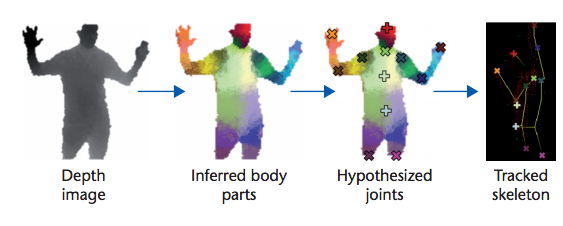
\includegraphics[scale=0.5]{zscreenshots/skeletonJoints.png}
    \caption{The Kinect Skeletal Tracking Pipeline}
\end{figure}